\newpage
\section{RESULT}
\subsection{Big Five Personality Frequency Distribution}
myPersonality dataset contains status updates of 223 users. These users come under Big Five Personality traits. We analyzed this data to see how users are distributed under different personality traits. The frequency distribution of each class of personality traits is given below:
\begin{figure}[!ht]
\centering
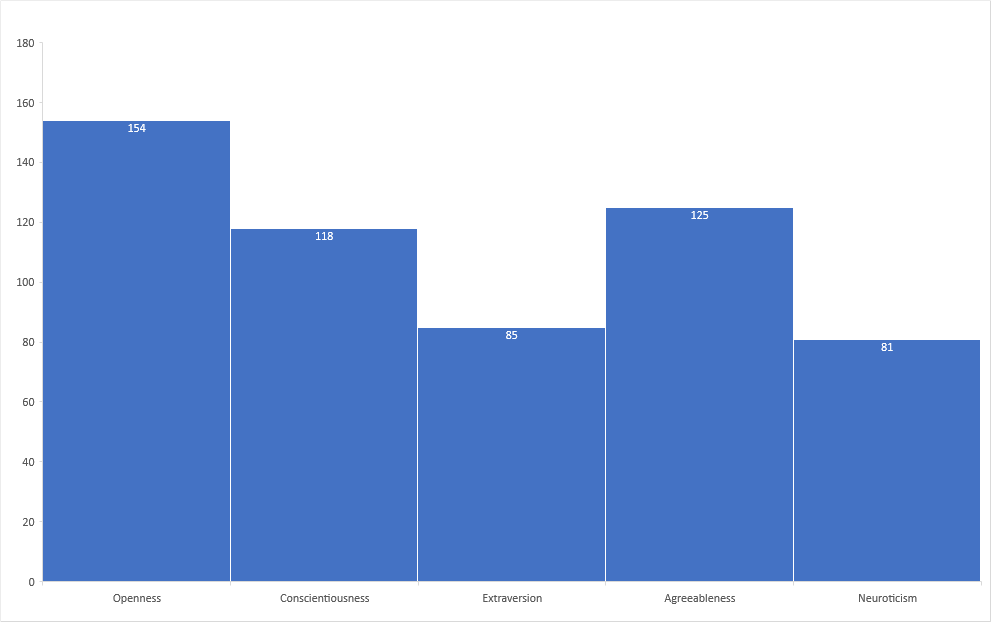
\includegraphics[width = \textwidth ]{fig/class_frequency.png}
\caption{Class Frequency Distribution of Users}
\label{fig:class_frequency}
\end{figure}

\subsection{Logistic Regression Model}
We analyzed the effect of number of iterations on the f-measure of the logistic regression model which is given below:
\begin{figure}[!ht]
\centering
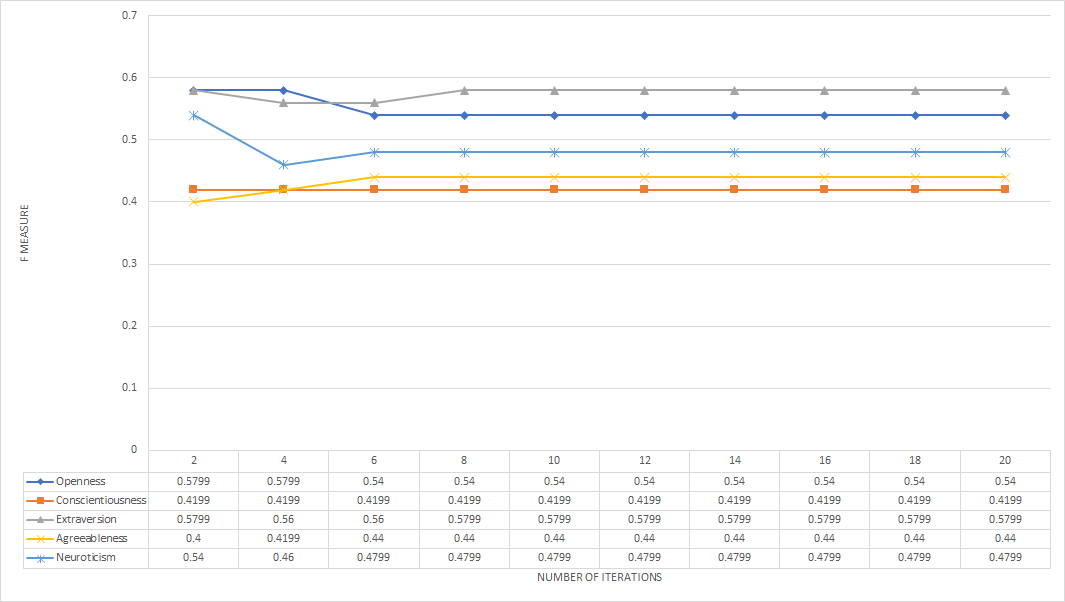
\includegraphics[width = \textwidth ]{fig/f-measure_logistic.png}
\caption{f-measure vs number of iterations (logistic regression)}
\label{fig:f-measure_logistic}
\end{figure}


The followings tables show the confusion matrix of Naive Bayes for Big Five Personality classes:
\begin{table}[!ht]
\centering
\begin{tabular}{ |c|c|c| } 
 \hline
 N =50 & Predicted:Yes & Predicted: No \\
 \hline
 Actual:Yes&4 & 11 \\ 
 \hline
 Actual:No&12 & 23 \\ 
 \hline
\end{tabular}
\caption{Confusion matrix of Logistic Regression Model (Openness)}

\end{table}

\begin{table}[!ht]
\centering
\begin{tabular}{ |c|c|c| } 
 \hline
 N =50 & Predicted:Yes & Predicted: No \\
 \hline
 Actual:Yes&6 & 18 \\ 
 \hline
 Actual:No&11 & 15 \\ 
 \hline
\end{tabular}
\caption{Confusion matrix of Logistic Regression Model (Conscientiousness)}
\end{table}

\begin{table}[!ht]
\centering
\begin{tabular}{ |c|c|c| } 
 \hline
 N =50 & Predicted:Yes & Predicted: No \\
 \hline
 Actual:Yes&22 & 9 \\ 
 \hline
 Actual:No&12 & 7 \\ 
 \hline
\end{tabular}
 \caption{Confusion matrix of Logistic Regression Model (Extraversion)}
\end{table}

\begin{table}[!ht]
\centering
\begin{tabular}{ |c|c|c| } 
 \hline
 N =50 & Predicted:Yes & Predicted: No \\
 \hline
 Actual:Yes&9 & 14 \\ 
 \hline
 Actual:No&14 & 13 \\ 
 \hline
\end{tabular}
 \caption{Confusion matrix of Logistic Regression Model (Agreeableness)}
\end{table}

\begin{table}[!ht]
\centering
\begin{tabular}{ |c|c|c| } 
 \hline
 N =50 & Predicted:Yes & Predicted: No \\
 \hline
 Actual:Yes&16 & 14 \\ 
 \hline
 Actual:No&12 & 8 \\ 
 \hline
\end{tabular}
 \caption{Confusion matrix of Logistic Regression Model (Neuroticism)}
\end{table}


\subsection{Naive Bayes Model}
The following figure shows f-measure of the naive bayes model for Big Five Personality classes:
\begin{figure}[!ht]
\centering
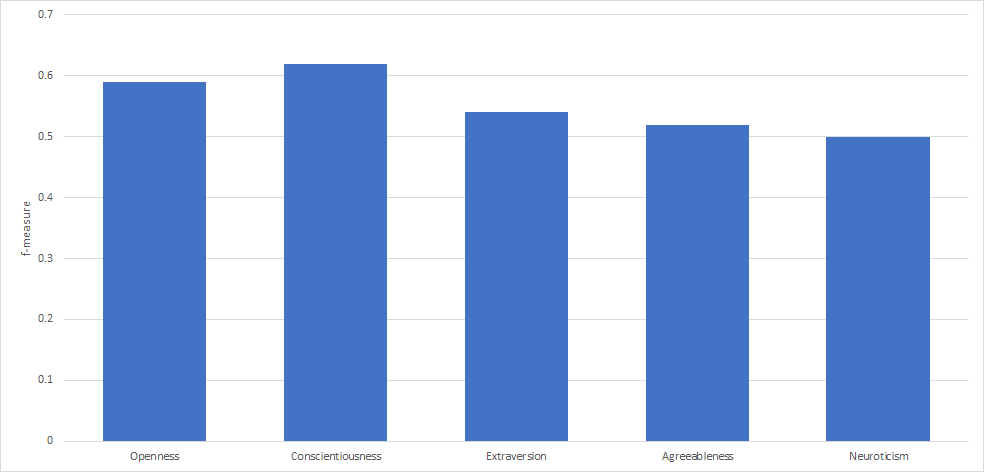
\includegraphics[width = \textwidth ]{fig/f-measure_naivebayes.png}
\caption{f-measure of Naive Bayes model}
\label{fig:f-measure_naivebayes}
\end{figure}

The followings tables show the confusion matrix of Naive Bayes for Big Five Personality classes:
\begin{table}[!ht]
\centering
\begin{tabular}{ |c|c|c| } 
 \hline
 N =50 & Predicted:Yes & Predicted: No \\
 \hline
 Actual:Yes&3 & 12 \\ 
 \hline
 Actual:No&8 & 27 \\ 
 \hline
\end{tabular}
\caption{Confusion matrix of Naive Bayes (Openness)}

\end{table}

\begin{table}[!ht]
\centering
\begin{tabular}{ |c|c|c| } 
 \hline
 N =50 & Predicted:Yes & Predicted: No \\
 \hline
 Actual:Yes&9 & 15 \\ 
 \hline
 Actual:No&4 & 22 \\ 
 \hline
\end{tabular}
\caption{Confusion matrix of Naive Bayes (Conscientiousness)}
\end{table}

\begin{table}[!ht]
\centering
\begin{tabular}{ |c|c|c| } 
 \hline
 N =50 & Predicted:Yes & Predicted: No \\
 \hline
 Actual:Yes&20 & 11 \\ 
 \hline
 Actual:No&12 & 7 \\ 
 \hline
\end{tabular}
 \caption{Confusion matrix of Naive Bayes (Extraversion)}
\end{table}

\begin{table}[!ht]
\centering
\begin{tabular}{ |c|c|c| } 
 \hline
 N =50 & Predicted:Yes & Predicted: No \\
 \hline
 Actual:Yes&12 & 11 \\ 
 \hline
 Actual:No&13 & 14 \\ 
 \hline
\end{tabular}
 \caption{Confusion matrix of Naive Bayes (Agreeableness)}
\end{table}

\begin{table}[!ht]
\centering
\begin{tabular}{ |c|c|c| } 
 \hline
 N =50 & Predicted:Yes & Predicted: No \\
 \hline
 Actual:Yes&20 & 10 \\ 
 \hline
 Actual:No&15 & 5 \\ 
 \hline
\end{tabular}
 \caption{Confusion matrix of Naive Bayes (Neuroticism)}
\end{table}


\subsection{Evaluation of Recommendation System}
RMSE of global baseline algorithm: \\
RMSE of user to user collaborative filtering with user rating matrix: \\
RMSE of user to user collaborative filtering with user personality matrix: \\
RMSE of user to user collaborative filtering with user rating matrix with combination of global baseline: \\
RMSE of user to user collaborative filtering with user personality matrix with combination of global baseline: \\
RMSE of user to user collaborative filtering with weighted average of user personality matrix and user rating matrix:\\
RMSE of user to user collaborative filtering with weighted average of user personality matrix and user rating matrix with combination of global baseline: \\
RMSE of matrix factorization: \\



\subsubsection{Latent Factor}
The following figure shows the RMSE of matrix factorization when number of iterations is varied:
\begin{figure}[!ht]
\centering
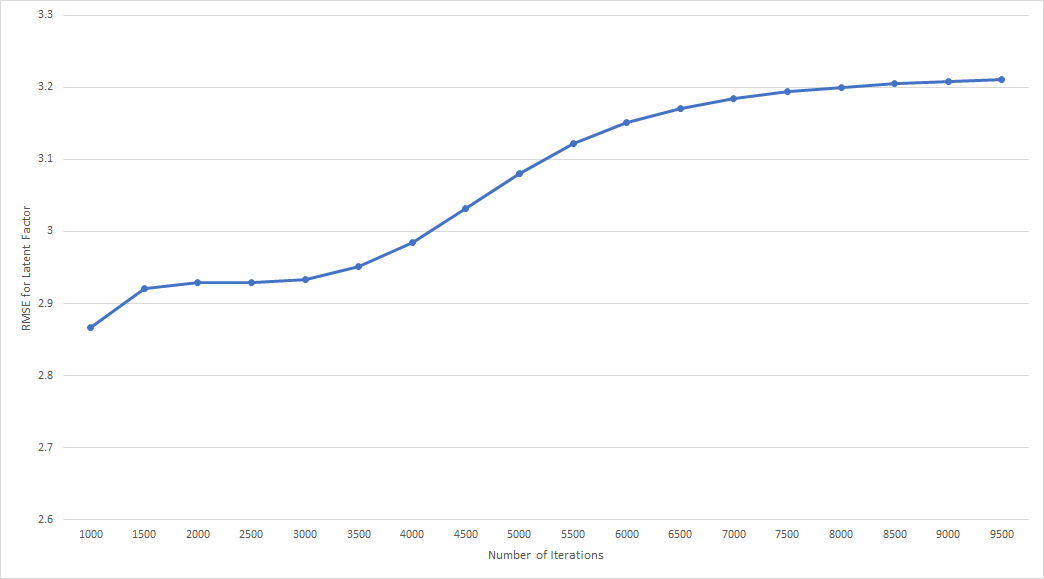
\includegraphics[width = \textwidth ]{fig/rmse_step.png}
\caption{RMSE of matrix factorization vs number of iterations}
\label{fig:rmse_step}
\end{figure}
\\
The following figure shows the RMSE of matrix factorization when k is varied with number of iterations is fixed at 1000:
\begin{figure}[!ht]
\centering
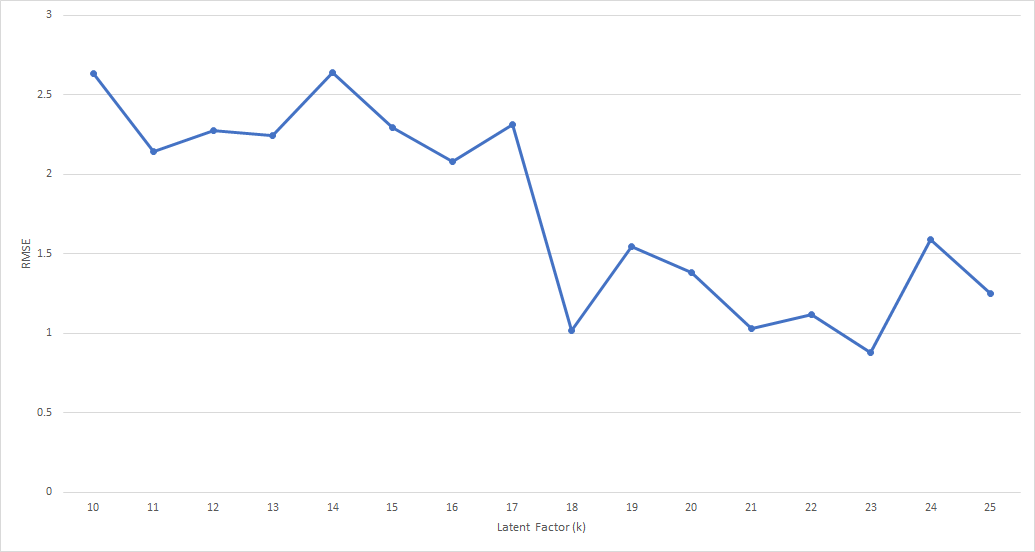
\includegraphics[width = \textwidth ]{fig/rmse_k.png}
\caption{RMSE of matrix factorization vs number of latent factors}
\label{fig:rmse_k}
\end{figure}